\chapter{PyHCL验证方法概述}

本章对PyHCL所包含的验证方法进行概述,包括基本单元测试使用的PyHCL-Tester、基于UVM的大规模集成测试框架PyUVM、以及在此基础上的针对RISC-V微处理器的差分测试框架。PyHCL所设计的验证方法是为了达到如下的目标:

\begin{enumerate}
	\item 填补其他硬件生成框架所缺乏的验证工具或方法。开发者可以通过PyHCL完成电路设计以及验证的全部过程,而不需要切换到其他的验证工具流或者语言。不包含有验证工具或方法的硬件生成框架存在一个难以解决的难题,那就是设计得到的代码要进行验证,则必须生成Verilog代码。常见的验证工具流仅支持Verilog或SystemVerilog代码的输入,而当基于高层次的电路表述编译为Verilog后,则通常会损失原设计中的信息,导致验证过程举步维艰。
	\item PyHCL的验证方法涵盖了各级别验证的粒度以及策略。在验证粒度方面,PyHCL涵盖了以单个模块为基准的单元测试到基于SoC片上系统的大规模集成测试。在验证策略方面,PyHCL支持白盒、黑盒以及灰盒测试。
	\item 支持UVM验证方法学。PyHCL包含基于Python而非SystemVerilog的大规模UVM验证平台PyUVM,支持验证复用以及随机向量测试的特性,同时也是实现本文微处理器的差分测试框架的基础。
\end{enumerate}

本章将介绍PyHCL验证方法中包括的主要模块:基于模块单元测试PyHCL-Tester、大规模集成测试框架PyUVM、针对第三章中实现的微处理器的差分测试框架。本章的最后将会给出各个PyHCL验证工具与当前流行的开源验证框架的性能对比。

\section{PyHCL-Tester与PyUVM}

PyHCL-Tester是PyHCL提供的基于模块单元测试的轻量级验证工具,PyHCL-Tester的内核基于开源的验证引擎Verilator[50],Verilator可以提供在开源验证工具当中最快的仿真速度。与基于Verilog Testbench的单元测试方法不同,PyHCL-Tester通过将Python仿真脚本内嵌在PyHCL电路RTL设计代码中实现,因此PyHCL-Tester可以给使用者带来快速的模块级的黑盒验证测试策略。相对于一些其他的基于Python的硬件生成框架,某些HGF会使用基于Python的仿真引擎来作为框架使用的验证工具,但是囿于Python固有的解释器解释执行而导致其性能较为平庸。 因此,PyHCL-Tester选择采用目前开源仿真引擎中最快的Verilator来作为内核,而Python-Tester则作为仿真的前端,通过管道的方式将仿真的数据以及指令通过自定义的协议发送给Verilator后端,并将Verilator后端的仿真结果再通过管道接收。图4-1展示了PyHCL-Tester以及结合FIRRTL执行器Treadle[51]的验证测试框架图。

\begin{figure}[htbp]
	\centering
	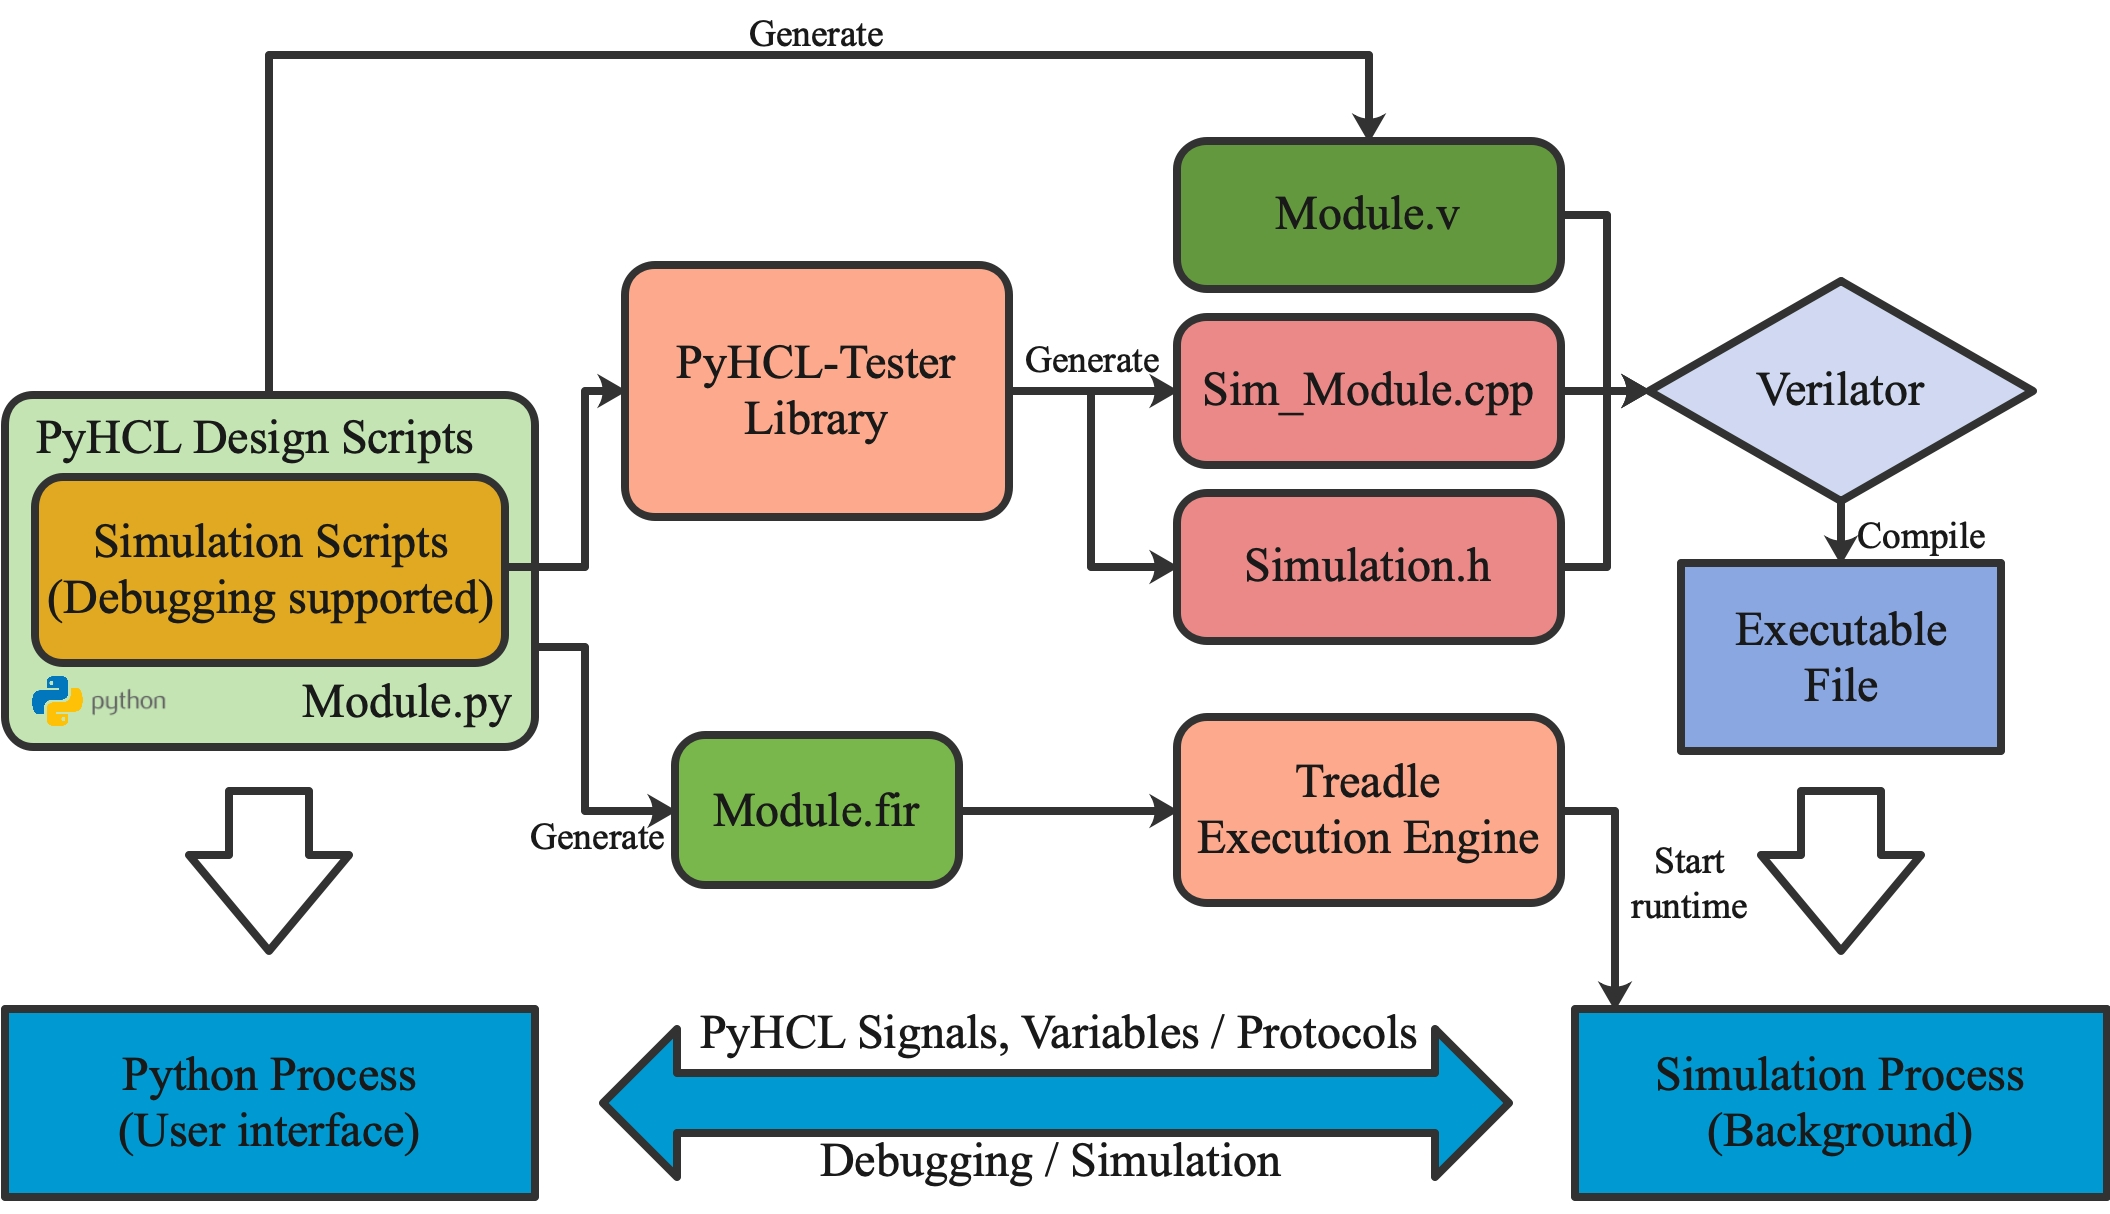
\includegraphics[width=0.95\textwidth]{Photos/PyHCL-Tester.jpg}
	\caption{PyHCL-Tester及Treadle的验证测试框架图}
\end{figure}

PyHCL-Tester库包含有生成C/C++仿真头文件所需要的基础模版,并提供若干个用户接口函数允许使用者基于2.1节中提供的PyHCL原语编写仿真脚本。举例来说,PyHCL-Tester中提供两个主要的接口来操纵所需要仿真的模块的IO端口:poke()用于提供给模块输入端口以激励,而peek()用于监测模块输出端口再各个时钟周期的输出信号变化,并通过该接口在仿真过程中实时返回给PyHCL-Tester前端。与传统的使用Verilog进行Testbench单元测试的方法不同,使用Verilog编写Testbench在对待测模块(Design Under Test,DUT)的单元测试代码时,激励的生成需要经过繁杂的时钟定义/生成、激励定义与描述的过程。而在PyHCL-Tester中,对输入端口的激励以及输出端口的监测可以直接指定模块对应的PyHCL原语,且激励信号的值也可以直接使用Python内置数据类型,且对于较为复杂的激励信号也可以使用第三方的Python科学计算库来生成。PyHCL-Tester的仿真脚本内嵌到PyHCL电路设计代码中,当仿真开始后,PyHCL电路设计部分的代码通过PyHCL及FIRRTL编译器生成Verilog代码,而内嵌在其中的PyHCL-Tester仿真脚本则生成作为Verilator输入的C/C++仿真头文件,这其中包含有预定义的管道以及通信协议结构代码。在这之后,电路RTL设计代码(Verilog)以及C/C++仿真头文件作为Verilator的输入进行编译,Verilator将Verilog描述的RTL级电路编译成等效的并发C/C++模型,最终生成对应的后台仿真可执行文件。当用户启动仿真时,前端的PyHCL-Tester仿真脚本进程调用后台生成的可执行文件作为后台仿真进程,两个进程之间通过管道以及预定义好的协议进行通信,协议主要定义了后端仿真进程的控制信号,如时钟周期步进、仿真启停等,前端PyHCL-Tester仿真脚本进程提供输入信号激励传递到后台C/C++仿真进程,时钟周期步进后,后台C/C++仿真进程返回模块输出端口信号的值到前端PyHCL-Tester仿真脚本。对于使用者来说,信号激励的输入与输出返回都是基于Python内置数据类型的,而不需要了解内在的仿真机理。因此,通过这种将电路设计以及仿真验证放在同一个接口层次的设计模式,PyHCL-Tester可以快速进行单个模块的单元验证测试,同时,PyHCL-Tester在性能方面与Verilator基本持平。

PyHCL-Tester也存在一定的缺点,虽然PyHCL-Tester在仿真性能上非常突出,但是对于大规模的系统级测试需要耗费大量额外的时间来编译仿真环境,因此PyHCL-Tester仅适合在小规模的单元测试中使用。此外,PyHCL-Tester使用黑盒的验证策略,因为PyHCL-Tester仅支持对模块的输入输出端口进行交互,而模块内部的信号情况是未知的。当测试出现错误时,是无法精确定位具体的电路逻辑的。为了解决该问题,PyHCL提供了一种辅助手段支持单元测试:Treadle。Treadle是一个FIRRTL的执行器,可以直接读取FIRRTL级的电路设计,并在仿真运行时返回内部所有信号如寄存器、线网的当前值。当前设计出现问题时,可以将后端的C/C++仿真进程切换到Treadle,并直接执行对应PyHCL电路RTL代码所生成的FIRRTL代码。用户使用相同的接口函数来为Treadle提供输入信号激励,并获取输出信号的值。与Verilator不同,使用Treadle可以在各个周期获取到模块内部信号的值,这种方式类似于调试中的断点,可以精确定位到出现问题的时钟周期以及模块内部具体的寄存器或者线网。Treadle所提供的验证策略属于白盒验证策略,DUT模块在仿真过程中会暴露所有内部信号的值。虽然Treadle可以提供相当详细的运行时信息,但是其缺点在于仿真的性能较差。因此使用PyHCL进行单元测试过程中,明智的做法是结合PyHCL-Tester以及Treadle使用。

PyHCL提供PyHCL-Tester作为单元测试以及小规模的功能测试使用。而对于大规模的系统级验证测试或SoC平台的集成测试,验证测试环境更需要考虑可重用性的问题。模块级的单元测试需要监测验证模块所有输入输出端口的值与参考模型的行为是否一致,而系统级的测试则专注于在实际的应用场景中系统中各个不同模块之间的交互。UVM验证方法学广泛应用在系统级的验证当中,其主要的验证思路是验证环境重用以及随机测试。但绝大多数的硬件生成框架都不支持基于UVM的验证环境,基于这些硬件生成框架的电路设计在需要进行大规模UVM验证时,都需要基于SystemVerilog重新搭建UVM测试平台,这将会导致设计与验证之间完全分隔开来,不利于硬件敏捷设计方法的应用。为了解决这一问题,PyHCL引入了支持UVM验证方法学的验证平台PyUVM。

PyUVM主要基于协程的开源协同仿真测试环境cocotb[52]搭建,cocotb允许使用者通过Python搭建基于UVM的验证测试环境。使用Python而非SystemVerilog来搭建UVM验证测试环境具有许多优势,如在Python中定义UVM测试中所需要使用的参考模型相比于使用SystemVerilog来说要相对简便很多。参考模型用于模拟实现相关算法的电路行为,UVM验证环境通过比对电路仿真验证以及参考模型的结果来验证DUT的设计是否符合规范。SystemVerilog一般需要导入外部的C/C++算法模型作为参考模型使用,而在PyUVM中则可以直接使用Python来对参考模型进行建模。此外,由于Python自身的解释执行特性,所有在PyUVM中的Python测试协程都可以在验证过程中随时修改并重启,而不需要重新编译耗费大量的时间,而Verilator则在对仿真头文件发生更改后,都需要重新进行编译。

基于cocotb的PyUVM的测试协程通过函数装饰器实现,cocotb包含一个对协程的调度器来调度不同测试协程的运行。与其他基于SystemVerilog的UVM验证框架不同,PyUVM不需要编写额外的RTL级验证代码。PyUVM同时支持多种后端的仿真引擎,包括Verilator、Icarus Verilog[53]、ModelSim等等。然而,PyUVM也存在一定的缺点,它使用VPI(Verilog Procedural Interface)作为Python构建的UVM验证测试环境与仿真器的交互接口,会带来一定的额外性能损耗。表4-1对PyHCL所提供的三种验证方法及工具进行了总结与对比。

\begin{table}
	\caption{PyHCL提供的三种验证方法及工具的对比}
	\centering
	\small 
	\begin{tabular}{cccc}
		\hline 
		特性 & PyHCL-Tester                & Treadle & PyUVM            \tabularnewline
		\hline 
		验证粒度级别   & 模块级		     & 模块级   & 系统级 \tabularnewline
		验证策略   & 黑盒		     & 白盒   & 黑盒 \tabularnewline
		可重用性   & 低		     & 低   & 很高 \tabularnewline
		仿真性能   & 高		     & 很低   & 中等 \tabularnewline
		参考模型复杂度   & 低		     & 无   & 高 \tabularnewline
		定位设计错误的难度   & 高		     & 很低   & 高 \tabularnewline
		开发验证环境所需的工作量   & 低		     & 低   & 高 \tabularnewline
		\hline 
	\end{tabular}
\end{table}

\section{基于多级验证环境的差分测试框架}

本小节介绍结合PyHCL所提供的三种验证测试方法所搭建的针对本文所实现微处理器的多级验证差分测试框架与环境。在4.1节中提到,PyHCL提供了三种不同的验证测试方法,从表5中可以发现,每种方法都有各自的利弊。为了充分发挥每种验证测试方法的优点,本文搭建了结合上述三种验证测试方法的多级验证测试环境,并在其中实现了一个针对第三章中实现的RV32GCP处理器的差分测试框架。该多级验证测试环境涵盖所有的验证粒度级别以及验证策略,包括灰盒验证策略。灰盒验证策略允许用户在保证仿真性能以及验证可重用性的同时,还可以快速定位到设计逻辑中的错误。该多级验证环境还可以轻松地与PyHCL实现的电路设计交互,这是因为4.1节中提到的PyHCL提供的三种验证方法都具有通用的接口,可以直接加载PyHCL设计并操作设计中的PyHCL电路实体原语。此外,该多级验证环境还可以通过Python导入外部的包或工具。同时,该多级验证环境通过若干通用可配置的模块组成,这些模块可以在整个设计和验证过程中重用,而不需要任何重大的修改,这种设计模式可以显著缩短开发周期。

图4-2给出了基于该多级验证环境的差分测试框架结构图。该多级验证环境基于cocotb来进行构建,这是因为cocotb带有原生的Python UVM验证方法支持。该多级验证环境可以分割成四个主要模块:使用PyHCL描述的待验证电路(DUT)、参考模型、仿真引擎以及前端的Python接口。在针对本文实现微处理器的差分测试框架中,DUT是RV32GCP的微处理器内核。参考模型是主流的RISC-V模拟器QEMU[54]或NEMU[55]。差分测试的主要思想就是对于根据同一种规范的两种实现,给定相同的有定义的输入,它们产生的行为应该一种。对于本差分测试框架,两种实现指的就是本文实现的RV32GCP微处理器软核以及RISC-V模拟器QEMU或NEMU。NEMU是QEMU的简化版本,两者的主要目的是使用C/C++代码来模拟一个单核或多核RISC-V处理器的行为。多级验证测试环境中实现了两种混合的验证测试方法:PyHCL-Tester+Treadle以及PyHCL-Tester+PyUVM,前者应用在模块级的单元测试当中,后者应用在系统级的大规模差分测试当中。其中PyHCL-Tester+PyUVM的方法使用默认的Icarus Verilolg仿真引擎,前端的Python接口用于与使用者进行交互。

\begin{figure}[htbp]
	\centering
	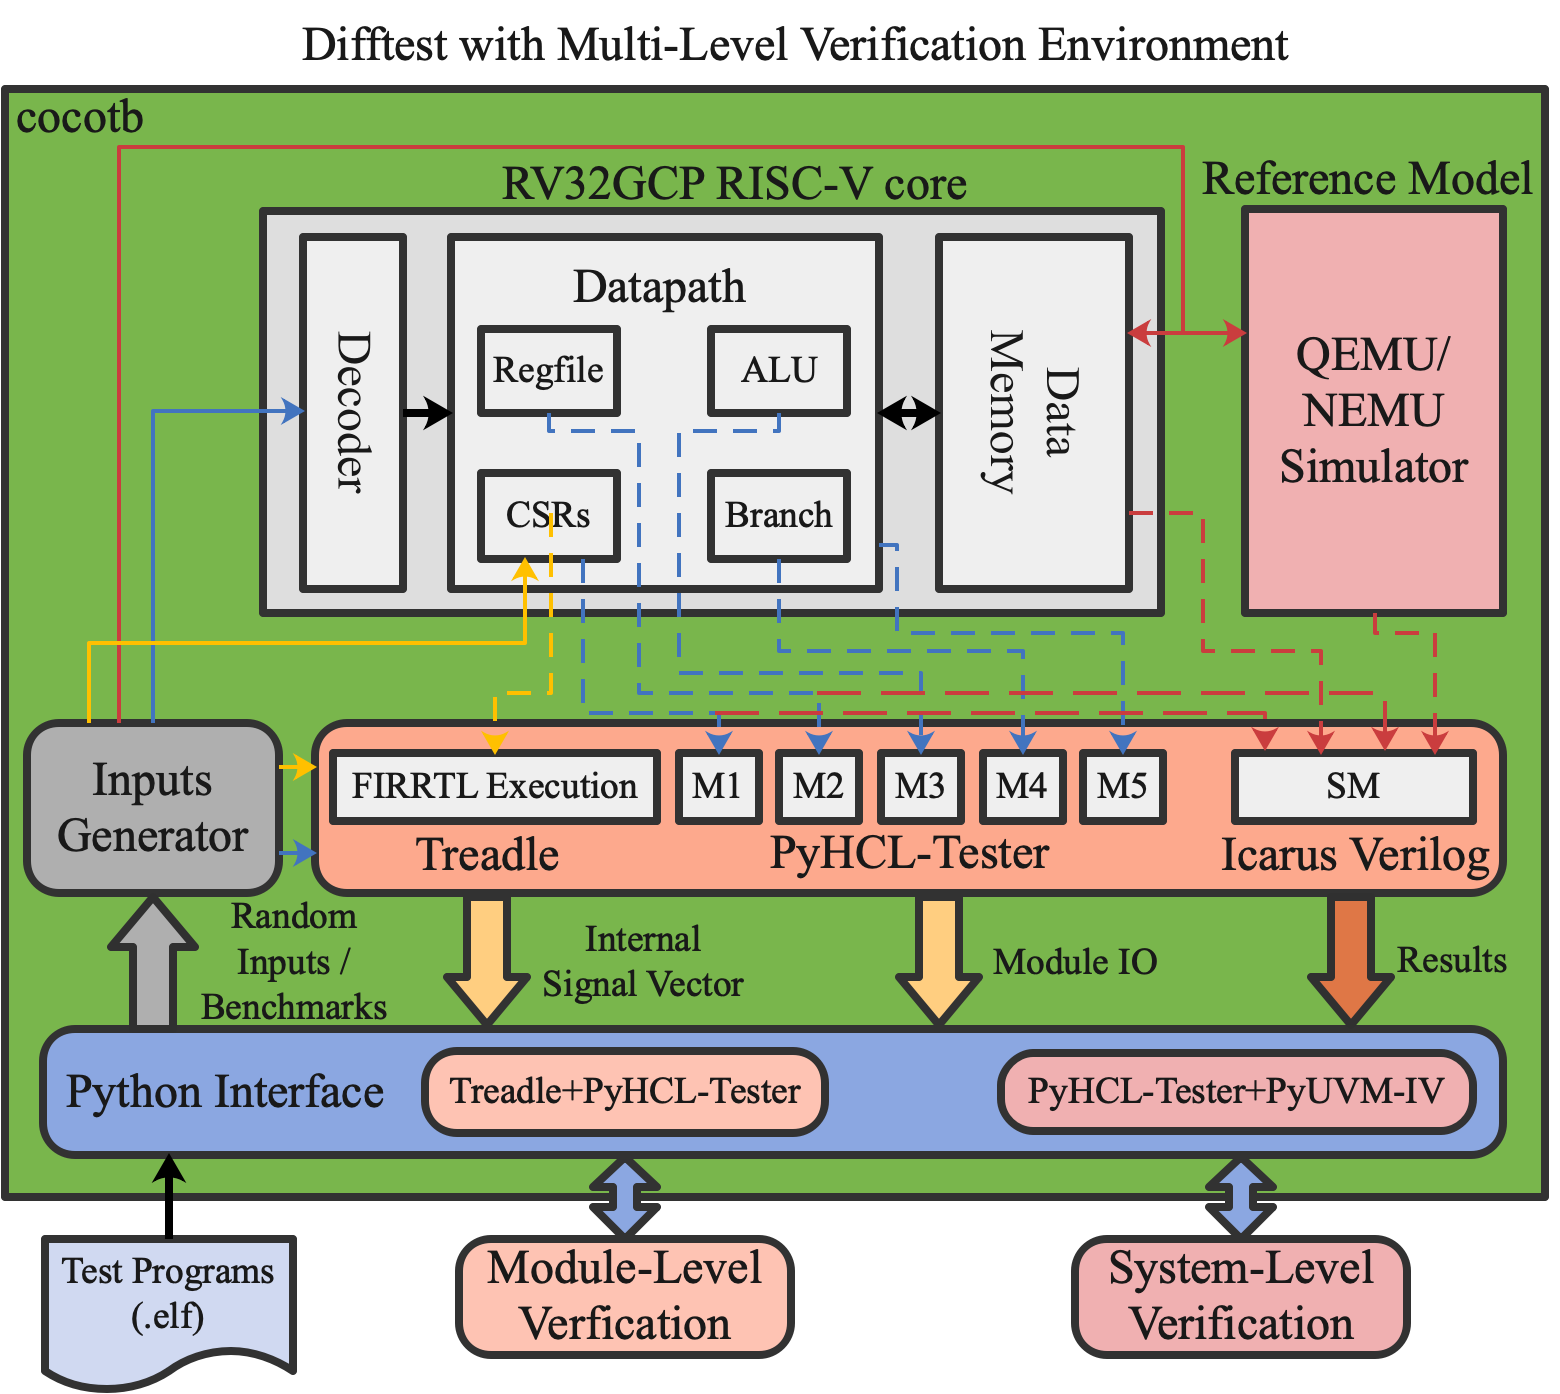
\includegraphics[width=0.95\textwidth]{Photos/multi-level-ve.png}
	\caption{基于多级验证环境的差分测试框架结构图}
\end{figure}

当使用该多级验证环境对本文所实现的RV32GCP微处理器进行验证时,首先从验证粒度较小的模块级单元测试开始。举例来说,当验证控制状态寄存器组CSRs单个模块时,多级验证环境使用PyHCL-Tester混合Treadle的验证方法。在图20当中使用黄色以及蓝色的箭头来分别表示Treadle以及PyHCL-Tester的数据流,实线代表输入数据,虚线代表输出数据。为了达到单个模块灰盒测试的目的,该方法使用PyHCL-Tester来监控模块的输出,与此同时在执行设计生成的FIRRTL代码的Treadle中插入若干断言。当Treadle执行到这些断言时,就会触发断点并返回当前模块内部信号值组成的向量。为了测试CSRs设计的正确性以及鲁棒性,多级验证环境会提供大量自定义或者随机生成的输入信号,并同时作为PyHCL-Tester以及Treadle的输入激励。此时用户可以通过PyHCL-Tester中对模块输出信号的监控单元来与模块级参考模型进行对比,来查看设计是否出错。需要注意的是,模块级的参考模型需要用户自定义,而非通过QEMU或NEMU,后者仅使用在大规模的差分测试当中。在图7中,这些监控单元使用MX来表示。如果模块的输出发现问题,用户可以随时切换到Treadle执行器,执行出现问题前后的若干时钟周期的的一小段仿真过程,根据断言返回的内部信号向量来定位PyHCL电路逻辑设计中产生的问题。Treadle在执行短周期仿真的性能与PyHCL-Tester并没有太大的区别。这种方法的关键点在于,结合PyHCL-Tester仿真的高性能以及Treadle定位设计错误的简便性,来达到在模块级单元测试中的灰盒验证目的。这种思路可以扩展到子系统级的功能验证,如针对条件分支的功能验证。在这种情况下,我们可以预先定义若干个包含条件分支的RISC-V汇编代码片段来作为译码器的输入,并使用PyHCL-Tester来观察若干模块的输出信号。如果输出信号发生错误,则首先根据不同的监控单元定位出错的模块。当问题模块被定为后,则可以切换到模块级单元测试的验证方法PyHCL-Tester+Treadle,来定位模块内部PyHCL电路逻辑设计中的错误。

当微处理器内核原型系统设计完成后,微处理器内核中的子模块都已经通过单元测试。此时多级验证平台将对整个微处理器核进行大规模的系统级测试。系统级的验证测试主要使用差分测试框架来完成,差分测试的实现主要通过将相同的RISC-V测试代码片段同时作为RV32GCP以及QEMU/NEMU模拟器的输入,在执行后,通过比对模拟器以及微处理器软核的处理器架构状态来查看微处理器是否存在逻辑错误。微处理器架构状态包括通用寄存器组、状态控制寄存器组CSRs、数据存储。作为输入的RISC-V测试代码可以使用随机指令生成框架如riscv-torture[56]或者是预定义的RISC-V标准测试例程如riscv-tests。测试代码通过Python接口导入到RV32GCP内核以及QEMU/NEMU模拟器的指令存储器当中。在测试代码的执行过程中,PyUVM的模拟器监控单元SM在每个时钟周期会实时比对微处理器内核与模拟器通用寄存器组的值,当出现差异时就会立刻抛出异常,并返回当前出错的指令以及时钟周期。对于riscv-tests,在测试代码执行完成后,还会检查存储器特定地址区域之间的差异,这是因为riscv-tests通过在数据存储特定地址写入若干标记,在测试例程结束后通过检查存储区目标地址微处理器是否存在与模拟器相同的标记即可判断测试是否通过。该基于Python的差分测试框架相对于基于SystemVerilog实现的差分测试框架性能要更好,这是因为SystemVerilog实现的差分测试框架,在编译后都会变成事件和队列的模型,并以事件驱动的方式来运行,因此本多级验证环境中基于Python实现的差分测试框架可以在测试运行时同时对比通用寄存器组值并即时抛出异常,而不会造成错误继续传播,造成调试的困难。

差分测试框架不单止使用了基于PyUVM的Icarus Verilog引擎进行验证测试,在本多级验证环境中还结合了PyHCL-Tester辅助测试代码的验证过程。当测试代码验证过程中抛出异常后,若发现错误来自于某特定的模块,则需要PyHCL-Tester介入。如果对单个模块使用PyUVM来重新执行测试代码,如4.1节中提到了,基于cocotb的PyUVM由于使用了VPI接口,在执行单模块的大量指令测试时会产生大量的额外开销。由于在单元测试中已经使用了PyHCL-Tester对各模块构建并编译了对应的监控单元,因此在大规模集成验证测试中可以重用这些已经编译好的C/C++仿真头文件,来监控测试代码执行过程中在异常指令附近该模块的输出信号是否有异常。PyUVM+PyHCL-Tester的方式可以作为大规模验证测试的灰盒验证策略,PyUVM可以快速构建差分测试平台并进行实时通用寄存器组的检查与对比,但无法得知具体模块的信号输出情况,而PyHCL-Tester可以提供该信息,以在保持性能的情况下得知微处理器内核内部的信号情况。

本节所实现的多级验证测试环境在对LeNet-5[57]以及VTA[58]等加速器软核实现中亦进行相关的验证测试,以确保该验证环境在异构系统中的适用性。本节所实现的多级验证测试环境的结果将在4.3节中给出。此外,本节中所实现的多级验证测试环境也是组成本文微处理器开发流程中的重要组成部分,可以加速对RV32GCP微处理器的验证过程,从而缩短每个功能的迭代开发流程,在第五章将会给出对本文所实现微处理器的硬件敏捷开发模型。

\section{PyHCL验证工具性能对比}

本节将对PyHCL中所提供的验证工具以及方法进行性能对比。表4-2给出了除本文实现的微处理器外到目前为止使用PyHCL实现的其他电路结构在Xilinx Artix 7 XC7A200T FPGA开发版上的综合情况,该开发版包含有215360个LUT,269200个可配置的触发器,740个DSP单元以及13150kb大小的BRAM。

\begin{table}
	\caption{使用PyHCL的电路RTL实现在Artix 7 FPGA开发板上的资源占用情况以及最大时钟频率}
	\centering
	\begin{tabular}{cccccc}
		\toprule
		\multirow{2}[2]{*}{设计} & \multicolumn{4}{c}{硬件资源使用} & \multicolumn{1}{c}{\multirow{2}[2]{*}{最大时钟频率 (MHz)}} \\
		\cmidrule{2-5}          & LUTs  & FFs   & DSPs  & \multicolumn{1}{c}{BRAM (bits)} &  \\
		\midrule
		RV32I Pipeline & 1004  & 441   & -     & 32K   & 141 \\
		LeNet-5 Accelerator & 18341 & 6877  & 144   & 768K  & 148 \\
		PicoRV32 & 879   & 578   & -     & 32K   & 243 \\
		VTA   & 40879 & 8689  & 114   & 3648K & 79 \\
		AXI4-Full & 191   & 224   & -     & -     & 294 \\
		Wallace Tree Multiplier & 50    & -     & -     & -     & 400 \\
		\bottomrule
	\end{tabular}%
\end{table}%

RV32IMC流水线是一个极小型的实验性RISC-V内核实现,是本文实现的RV32GCP微处理器的前身。PicoRV32是在第1.1.2节中提到的面向FPGA面积优化的RISC-V内核实现。LeNet-5加速器是对经典手写数字分类识别神经网络LeNet-5的硬件加速实。VTA是一个可编程的加速器架构,是TVM[59]架构的硬件扩展之一,可以借助TVM的上层工具链,构成端到端的深度学习加速器解决方案。PicoRV32以及VTA为使用PyHCL重构后综合得到的结果。AXI4是对AMBA AXI4主从端的逻辑实现。在最后还给出了使用PyHCL实现的基于华莱士树的乘法器综合结果。

表4-3给出了PyUVM中提供的三种验证方法及工具与Verilator仿真验证的性能的对比,其中PyUVM使用默认的Icarus Verilog仿真引擎。仿真验证测试的电路软核设计与表4-2相同。测试中使用的Verilator版本为4.034,Icarus Verilog版本为10.3,cocotb版本为1.3.2。每种方法测试数据通过10次重复测试取平均值得到,每次测试仿真执行10万个时钟周期。

\begin{table}
	\caption{PyHCL验证测试工具性能 (单位:秒)}
	\centering
	\begin{tabular}{ccccc}
		\toprule
		\multicolumn{1}{c}{设计} & PyHCL-Tester& PyUVM - Icarus Verilog & Treadle & Verilator \\
		\midrule
		RV32IMC流水线 & 0.78  & 15.81  & 29.36  & 0.79  \\
		LeNet-5加速器 & 5.70  & 28.64  & 175.74  & 5.60  \\
		PicoRV32 & 0.12  & 12.97  & 8.16  & 0.13  \\
		VTA   & 6.29  & 35.03  & 296.16  & 6.17  \\
		AXI4主从端 & 0.08  & 12.85  & 4.60  & 0.09  \\
		华莱士树乘法器 & 0.06  & 12.04  & 1.12  & 0.07  \\
		\bottomrule
	\end{tabular}%
\end{table}%

从表4-3中,可以发现PyHCL-Tester的性能与Verilator接近,这是因为两者都是以轻量级高速仿真为目标的仿真器。然而,两者都有相同的缺点:PyHCL-Tester以及Verilator都不支持模块内部信号的监控。而Treadle可以在运行时保存模块内部所有信号的值,因此可以随时获取模块内部信号在当前周期的值,然而代价是相对较差的性能。在相同条件下,Treadle相比PyHCL-Tester的仿真时间平均要慢38倍,最慢要达到67倍。但同时也要注意到在小模块的仿真,如华莱士乘法树当中,Treadle的仿真时间还处于可以接受的范围内。对于PyUVM,在验证测试时通常使用默认的Icarus Verilog仿真引擎,因为其比Verilator要更稳定。可以发现,PyUVM的仿真性能介于PyHCL-Tester以及Treadle之间,且具有最为稳定的仿真验证性能表现:对于PyHCL-Tester以及Treadle,最长仿真时间与最短仿真时间的比值为105以及264。然而对于使用Icarus Verilog的PyUVM,最长仿真时间与最短仿真时间的比值约为3。

从表4-3可以得出,PyHCL所提供的所有单个验证方法或工具应用在每种验证场景中都有一定的尴尬之处。对于PyHCL-Tester来说,其具有最佳的仿真验证性能,但无法获取模块内部的信号值信息。同时,PyHCL-Tester相比PyUVM在大规模的集成测试中需要耗费大量时间编译验证环境,此外,PyHCL-Tester还不具有验证环境的重用性。对于Treadle来说,它在运行时保存有模块所有内部信号的信息,但因此需要承受较低仿真性能的代价。对于PyUVM来说,通过使用Icarus Verilog仿真引擎可以达到最为稳定的仿真性能表现,但是在小模块的仿真时会带来额外的性能损耗。为了解决上述问题,在4.2节中多级验证测试环境中所提出的两种混合的仿真测试方法:PyHCL-Tester+Treadle以及PyUVM+PyHCL-Tester,两者分别应用在模块级单元测试以及大规模的集成测试中。表4-4给出该多级仿真验证环境中所有验证方法的性能,包括3种单个验证方法以及2个混合的验证方法。对于模块级的单元测试,本文从RV32GCP的微处理器核中提取CSRs以及ALU两个模块以及VTA的取指单元进行测试。对于大规模的系统级测试,本文选用RV32IMC的流水线、LeNet-5以及VTA加速器进行测试。

对于模块级的单元测试,PyHCL-Tester+Treadle的性能要显著优于Treadle,带来平均63\%的性能提升,且仿真的时间也平均只比PyHCL-Tester要慢9倍左右,对于单模块的测试上来说,基本上都在1s的时间浮动,这对于模块级的单元测试来说是可以接受的。与此同时,使用该方法还可以在仿真同时获取模块内部的信号值信息。对于大规模的系统级验证测试,PyUVM+PyHCL-Tester的性能要比PyUVM带来平均40\%的性能提升。PyUVM+PyHCL-Tester的性能虽然逊于PyHCL-Tester,但在大型电路设计项目上,如VTA以及LeNet-5上两者的性能差距要更小。对于大规模项目来说,这种差距也是可接受的。此外,PyUVM+PyHCL-Tester在大规模系统级验证测试上的稳定性要优于PyHCL-Tester,前者最长仿真时间与最短仿真时间的比值为1.7,而后者则达到8。

\begin{table}
	\centering
	\caption{多级验证环境的仿真性能(单位:秒)}
	\begin{tabular}{ccccccc}
		\toprule
		验证粒度级别 & 设计 & Py-T & TDL & PyUVM-IV & PT+TDL & PU-IV+PT\\
		\midrule
		\multirow{3}[1]{*}{模块级} & RV32IMC CSRs & 0.14  & 4.53  & -     & \textbf{0.59 } & - \\
		& RV32IMC ALU & 0.06  & 0.87  & -     & \textbf{0.42 } & - \\
		& VTA 取指单元 & 0.09  & 3.51  & -     & \textbf{1.79 } & - \\
		\midrule
		\multirow{3}[1]{*}{系统级} & RV32IMC流水线 & 0.81  & -     & 18.53  & -     & \textbf{10.96 } \\
		& LeNet-5加速器 & 5.67  & -     & 27.07  & -     & \textbf{17.26 } \\
		& VTA   & 6.30  & -     & 33.63  & -     & \textbf{18.80 } \\
		\bottomrule
	\end{tabular}%

\begin{threeparttable}
	\begin{tablenotes}
		\linespread{1.4}
		\footnotesize
		\item Py-T = PyHCL-Tester
		\item TDL = Treadle
		\item PyUVM-IV = PyUVM with Icarus Verilog
		\item PT+TDL = PyHCL-Tester + Treadle
		\item PU-IV+PT = PyUVM with Icarus Verilog + PyHCL-Tester
	\end{tablenotes}
\end{threeparttable}
\end{table}%

\begin{table}
	\caption{不同验证方法构建验证环境时间的对比(单位:秒)}
	\centering
	\begin{tabular}{cccc}
		\toprule
		设计 & PyHCL-Tester & PU-IV+PT* & PyUVM-IV \\
		\midrule
		RV32I Pipeline & 3.66  & 0.62 & 0.67  \\
		LeNet-5 Accelerator & 6.05  & 3.16 & 3.07  \\
		VTA   & 8.87  & 2.80 & 2.64  \\
		\bottomrule
	\end{tabular}%
	
	\begin{threeparttable}
		\begin{tablenotes}
			\linespread{1.4}
			\footnotesize
			\item[*] PyUVM with Icarus Verilog + PyHCL-Tester
		\end{tablenotes}
	\end{threeparttable}
\end{table}%

表4-5给出了PyHCL-Tester、PyUVM以及PyUVM+PyHCL-Tester的验证环境构建时间比较。测试的环境配置与仿真环境相同。可以发现,混合的PyUVM+PyHCL-Tester的构建时间比PyHCL-Tester要更快,而与PyUVM比较接近。PyUVM+PyHCL-Tester的构建时间平均比PyHCL-Tester要快66\%。除此之外,在验证环境发生改变时,PyHCL-Tester需要重新编译整个验证环境,而PyUVM+PyHCL-Tester则只需要动态编译改变的部分。

综上所述,本章中提出的两种混合的验证测试策略结合了单个不同验证方法的优势并保持了相对较高的仿真性能。对于模块级的单元测试,PyHCL-Tester+Treadle的混合策略可以在保持高仿真性能的同时精确定位模块内部的逻辑设计错误。对于大规模的集成测试,PyUVM+PyHCL-Tester的混合策略可以在保证可重用性以及较短仿真环境构建时间的同时,带来相对合理的仿真性能表现。

\section{本章小结}

本章对PyHCL所提供的三种验证方法与工具:PyHCL-Tester、Treadle以及PyUVM进行了介绍。为了解决这三种方法所存在的一些固有的缺点,在实现本文的RV32GCP微处理器过程中,构建了一个多级验证测试平台,并包含用于该微处理器的差分测试框架。在多级验证测试平台中,实现了两种混合的验证测试方法:PyHCL-Tester+Treadle以及PyUVM+PyHCL-Tester。该两种混合的验证测试方法在保证性能的前提下,前者在模块级测试中可以精确定位内部的设计逻辑错误,后者在大规模集成测试中可以保证短的验证环境构建时间以及可重用性,两者都实现了灰盒验证的策略。通过该多级验证测试平台,在开发本文的微处理器核过程中,可以显著缩短每个功能开发迭代周期的验证时间,加速开发迭代的周期。